
\documentclass[a4paper,12pt,Times]{article}
\usepackage{abakos}  %pacote com padrão da Abakos baseado no padrão da PUC

% Pacote para a definição de novas cores
\usepackage{xcolor}
% Definindo novas cores
\definecolor{verde}{rgb}{0.25,0.5,0.35}
\definecolor{jpurple}{rgb}{0.5,0,0.35}
\definecolor{darkgreen}{rgb}{0.0, 0.2, 0.13}
%\definecolor{oldmauve}{rgb}{0.4, 0.19, 0.28}
% Configurando layout para mostrar codigos Java
\usepackage{listings,newtxtt}

\lstset{basicstyle=\ttfamily, keywordstyle=\bfseries}

\lstset{%
  escapeinside={(*}{*)},%
}

\newcommand{\estiloJava}{
\lstset{
    language=Java,
    basicstyle=\ttfamily\small,
    keywordstyle=\color{jpurple}\bfseries,
    stringstyle=\color{red},
    commentstyle=\color{verde},
    morecomment=[s][\color{blue}]{/**}{*/},
    extendedchars=true,
    showspaces=false,
    showstringspaces=false,
    numbers=left,
    numberstyle=\tiny,
    breaklines=true,
    backgroundcolor=\color{cyan!10},
    breakautoindent=true,
    captionpos=b,
    xleftmargin=0pt,
    tabsize=2
}}

\newcommand{\estiloR}{
  \lstset{ %
    language=R,                     % the language of the code
    basicstyle=\footnotesize,       % the size of the fonts that are used for the code
    numbers=left,                   % where to put the line-numbers
    numberstyle=\tiny\color{gray},  % the style that is used for the line-numbers
    stepnumber=1,                   % the step between two line-numbers. If it's 1, each line
                                    % will be numbered
    numbersep=5pt,                  % how far the line-numbers are from the code
    backgroundcolor=\color{white},  % choose the background color. You must add \usepackage{color}
    showspaces=false,               % show spaces adding particular underscores
    showstringspaces=false,         % underline spaces within strings
    showtabs=false,                 % show tabs within strings adding particular underscores
    frame=single,                   % adds a frame around the code
    rulecolor=\color{black},        % if not set, the frame-color may be changed on line-breaks within not-black text (e.g. commens (green here))
    tabsize=2,                      % sets default tabsize to 2 spaces
    captionpos=b,                   % sets the caption-position to bottom
    breaklines=true,                % sets automatic line breaking
    breakatwhitespace=false,        % sets if automatic breaks should only happen at whitespace
    title=\lstname,                 % show the filename of files included with \lstinputlisting;
                                    % also try caption instead of title
    keywordstyle=\color{blue},      % keyword style
    commentstyle=\color{darkgreen},   % comment style
    stringstyle=\color{red},      % string literal style
    escapeinside={\%*}{*)},         % if you want to add a comment within your code
    morekeywords={*,...}          % if you want to add more keywords to the set
}}


\newcommand{\comment}[1]{}
\graphicspath{ {figuras/} }

%%%%%%%%%%%%%%%%%%%%%%%%%%%
%Capa da revista
%%%%%%%%%%%%%%%%%%%%%%%%%%
\clearpage
\setcounter{page}{1} %iniciar contador de pagina de valor especificado
\newcommand{\monog}{Reentrega da trabalho da matéria de Grafos Trabalho 2 - Caminhos}
\newcommand{\monogES}{}
\newcommand{\tipo}{Trabalho}  % Especificar a seção tipo do trabalho: Artigo, Resumo, Tese, Dociê etc
\newcommand{\origem}{Brasil }
\newcommand{\editorial}{Belo Horizonte, p. \thepage - \pageref{LastPage}, dez. 2021}  % p. xx-xx – páginas inicial-final do artigo
\newcommand{\lcc}{\scriptsize{Licença Creative Commons Attribution-NonCommercial-NoDerivs 3.0 Unported}}

%%%%%%%%%%%%%%%%%INFORMAÇÕES SOBRE AUTOR PRINCIPAL %%%%%%%%%%%%%%%%%%%%%%%%%%%%%%%
\newcommand{\AutorA}{Gustavo Torres Bretas Alves}
\newcommand{\funcaoA}{}
\newcommand{\emailA}{gtbalves@sga.pucminas.br}
\newcommand{\cursA}{Aluno do Programa de Graduação em Ciência da Computação}

\newcommand{\AutorB}{Silvio Jamil Ferzoli Guimarães}
\newcommand{\funcaoB}{}
\newcommand{\emailB}{}
\newcommand{\cursB}{Professor do Programa de Graduação em Ciência da Computação}

% Definir macros para o nome da Instituição, da Faculdade, etc.
\newcommand{\univ}{Pontifícia Universidade Católica de Minas Gerais}

\newcommand{\keyword}[1]{\textsf{#1}}

\begin{document}
% %%%%%%%%%%%%%%%%%%%%%%%%%%%%%%%%%%
% %% Pagina de titulo
% %%%%%%%%%%%%%%%%%%%%%%%%%%%%%%%%%%

\begin{center}

\includegraphics[scale=0.2]{figuras/brasao.jpg} \\
PONTIFÍCIA UNIVERSIDADE CATÓLICA DE MINAS GERAIS \\
Instituto de Ciências Exatas e de Informática

% \vspace{1.0cm}
 \vspace{0cm} {
 \singlespacing \Large{\monog \symbolfootnote[1]{Artigo apresentado ao Instituto de Ciências Exatas e Informática da Pontifícia Universidade Católica de Minas Gerais} \\ }
  \normalsize{\monogES}
 }

Trabalho reentregue na matéria de Grafos para reavaliação, relacionado ao \textbf{Trabalho 2 - Caminhos}
 
\end{center}
\vspace{1.0cm}
\begin{flushright}
\singlespacing 
\normalsize{\AutorA \footnote{\funcaoA \cursA, \origem -- \emailA . }} \\
\normalsize{\AutorB \footnote{\funcaoB \cursB, \origem -- \emailB . }} \\
\end{flushright}
\thispagestyle{empty}
\selectlanguage{brazilian}
\onehalfspace  % espaçamento 1.5 entre linhas
\setlength{\parindent}{1.25cm}

%%%%%%%%%%%%%%%%%%%%%%%%%%%%%%%%%%%%%%%%%%%%%%%%%
%% SUMÁRIO
%%%%%%%%%%%%%%%%%%%%%%%%%%%%%%%%%%%%%%%%%%%%%%%%%

\newpage
\tableofcontents
\newpage
%%%%%%%%%%%%%%%%%%%%%%%%%%%%%%%%%%%%%%%%%%%%%%%%%
%% INICIO DO TEXTO
%%%%%%%%%%%%%%%%%%%%%%%%%%%%%%%%%%%%%%%%%%%%%%%%%

\section{Justificativa de reentrega}

Estou enviando esse trabalho com o objetivo de apresentar o documento (em PDF e TEX) e um novo código fonte desenvolvido para o trabalho após entender sobre a correta aplicação de um método eficaz para o encontro dos caminhos disjuntos.

Pelos fatos citados acima e por ter enviado erroneamente um trabalho de outra matéria por desatenção na primeira entrega, refiz esse trabalho com o objetivo de apresenta-ló mais bem redigido, alcançando um melhor desempenho, desde formato de apresentação, formatação do documento, organização dos conteúdos e qualidade do código.

Agradeço pela compreensão e abertura para essa entrega da atividade repositiva.

\section{Contextualização}

Um caminho simples em um grafo direcionado é um caminho sem vértices repetidos. Mais precisamente, um caminho é uma sequência (v0, a1, v1, a2, v2, . . . , ak, vk) com k >= 1 em que v0, v1, v2, . . . , vk são distintos dois a dois. Em grafos simples, pode-se representar um caminho apenas pela sequência de vértices (uma vez que só pode existir uma única aresta entre cada par de vértices). No grafo ilustrado na Fig. 1 as sequências (A, B, E, F ) e (A, D, C, F ) são exemplos de caminhos simples. Além disso, esses dois caminhos são disjuntos em arestas pois não possuem nenhuma aresta em comum.

O problema de se determinar o número máximo de caminhos disjuntos em arestas existentes em um grafo apresenta várias aplicações. Neste trabalho você deverá implementar um método de resolução deste problema que receba um grafo e um par de vértices (isto é, origem e destino) exiba ao final a quantidade de caminhos disjuntos em arestas entre os dois vértices dados, além de listar cada um dos caminhos encontrados.
\\
\\
Numa lista de tarefas, devemos implementar no algoritmo as seguintes regras:

\begin{itemize}
  \item método de resolução deste problema que receba um grafo e um par de vértices (isto é, origem e destino)
  \item exiba ao final a quantidade de caminhos disjuntos em arestas entre os dois vértices
  \item listar cada um dos caminhos encontrados.
\end{itemize}


% descrevendo detalhes da implementação, dos experimentos e resultados obtidos.

%xiba ao final a quantidade de caminhos disjuntos em arestas entre os dois vértices dados, além de listar cada um dos caminhos encontrados.

\subsection{Lógica}

Nesse trabalho devemos encontrar o número máximo de caminhos disjuntos em arestas existentes em um grafo. O código deve apresentar a quantidade de caminhos disjuntos em arestas entre os dois vértices dados e listar cada um dos caminhos encontrados.

Temos algumas formas de fazer essa busca, entretanto, algumas delas não são buscas consideradas ótimas, como é o caso do BFS com exclusão de arestas.

Como no caso do exemplo abaixo que chegamos do vértice D saindo do A e encontramos apenas um caminho "ótimo", visto o algoritmo.
\begin{center}
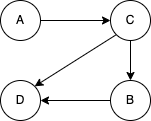
\includegraphics[width=5cm, height=4cm]{figuras/01.png}
\end{center}

\subsection{Lógica Ótima}
Pensando que devemos ter uma lógica ótima, devemos ter um algoritmo que não delete as arestas e que encontre e mostre o número máximo e atenda todas as expectativas.

Podemos então utilizar como base o algoritmo de fluxo em rede, como no caso do de Ford Fullkerson para realizar todas as tarefas e encontrar os caminhos disjuntos, mostrando-os e contabilizando-os.

\section{Definições}

\subsection{Par de caminhos disjuntos}
Um par de caminhos (por meio de vértices) em um grafo é considerado disjunto se e somente se não possuírem arestas em comum, ou seja, se nenhuma aresta do grafo é utiliza por ambos os caminhos.

Exemplo: No grafo definido abaixo, os caminhos (1,2,4) e (1,3,4) são disjuntos.  Já os caminhos (1,2,3,4) e (1,3,4) não são disjuntos.

\begin{center}
  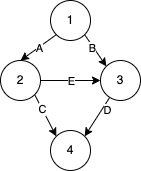
\includegraphics[ height=4cm]{figuras/02.png}
\end{center}


\subsection{Rede de Fluxo}
Uma rede de fluxo é um grafo direcionado G = (N, A), com N como conjunto de nós e A o conjunto de arestas, com as seguintes propriedades:
\\
\\
- Para cada aresta $a \in A$ há um número não negativo $C_{a}$, que indica a capacidade da mesma (ou seja, a quantidade máxima de fluxo que cada uma é capaz de carregar).\\
- Existe um único nó que será identificado como fonte (source), a ser denotado por s;\\
- Existe um único nó que será identificado como terminal (ou sumidouro) t, tal que $t \in N$;\\
- Não há nenhuma aresta direcionada para a fonte s, apenas arestas que saem dela e são direcionadas para outros nós.\\
- Não há nenhuma aresta que saia do terminal t, apenas arestas direcionadas a ele.


\section{Escolha do algoritmo}

\\

Para encontrar o número máximo de caminhos disjuntos podemos utilizar alguns algoritmos, entretanto como citado acima um deles é considerado ótimo. Ao escolher um BFS ou DFS como algoritmo alguns casos terão sucesso, porém em outros teremos erros que consideram caminhos disjuntos falsos, ou até mesmo a falta deles.
\\

Utilizei como base o algoritmo de Ford-Fulkerson para a solução do problema, utilizando como fluxo máximo em cada aresta começando em zero respeitando as seguintes propriedades:
\\
\\
Restrições de capacidade: Para cada $a \in A$, temos que $0 <= f(a) <= c_{a} $
\\
Restrições de conservação: Para cada nó $n \in N$ diferente de $s$ e $t$, temos que o fluxo total que entra em determinado nó é igual ao fluxo total que sai de tal nó.

\subsection{O algoritmo de Ford-Fulkerson}
Iniciamos supondo que o fluxo inicial em todas as arestas é nulo, e com isso iremos aumentar acrescentando fluxo na fonte com algumas regras.

A ideia principal do algoritmo gira em torno de duas principais operações:
\begin{itemize}
  \item Quando uma aresta tem menos fluxo do que permite a sua capacidade (incluindo o fluxo nulo), podemos "empurrar"  fluxo em sua direção.
\item Quando uma aresta tem uma quantidade positiva de fluxo, menor ou igual à sua capacidade, podemos fazer com que esse fluxo retroceda, "empurrando-o para trás"
\end{itemize}
\newpage
Para tais operações do algoritmo, devemos utilizar um grafo auxiliar, que segundo as questões já definidas chamaremos de \textbf{Grafo Residual ({$G_{R}$})} seguindo também algumas regras:


\begin{itemize}
  \item O conjunto de nós $G_{R}$ é o mesmo de $G$
  \item Ao percorrer as arestas em $G$, vamos criando as arestas de $G_{R}$ da seguinte maneira:
  \\\\
   - Para cada aresta $a = (n_{i},n_{j})$ de $G$ - (sai do nó $n_{i}$ e entra no nó $n_{j}$) - que possui fluxo $f(a) < c_{a}$, adicionamos uma aresta $a_{R} = (n_{i},n_{j})$ com capacidade $c_{aR}$ = $c_{a} - f(a) e f(a_{r})$ = 0. Deste modo, estamos definindo a possibilidade de "empurrar para frente" a quantidade de fluxo que a aresta $a$ conseguiria carregar a mais.
   \\\\
   - Para cada aresta $a = (n_{i},n_{j})$ de $G$ tal que $f(a) > 0$, ou seja, cada aresta que já esteja carregando alguma quantidade positiva de fluxo, existe a possibilidade de empurrar este fluxo para trás, se assim desejarmos. Desta forma, adicionamos uma aresta $a{'}_{R} = (n_{i},n_{j})$  em $G_{R}$ com direção inversa a $a$ e a capacidade $c_{a{'}_{R}} = f(a)$. Assim como no passo anterior, o fluxo de $a{'}_{R}$ no grafo residual é nulo.
\end{itemize}
\newpage



\section{Implementação}

\subsection{Detalhes da implementação}

Para a implementação do trabalho com objetivo de criar um método para resolver o problema de determinar o número máximo de caminhos disjuntos em arestas existentes em um grafo, utilizamos três principais pontos, dentre eles os três que serão explicados e deslindados abaixo.


% Matriz de adjacência
\subsubsection{Matriz de Adjacência}
Para inserir os grafos no algoritmo utilizamos matrizes de adjacências, utilizando sempre o peso 1 para as arestas, tendo como objetivo que cada aresta só pode ter um uso durante o encontro do caminho disjunto.

Exemplo de Matriz de Adjacência para o seguinte Grafo:

\begin{center}
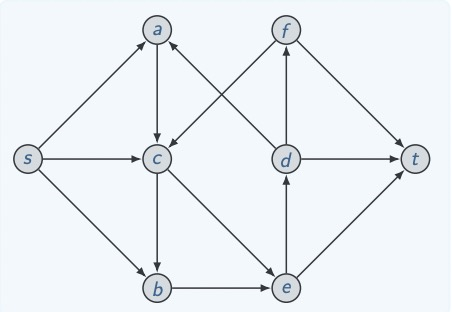
\includegraphics[height=4cm]{figuras/04.jpg}
\end{center}

\begin{scriptsize}
\estiloR
\begin{lstlisting}[title={Matriz de Adjacência para o Grafo acima}, label=lst:javacode]
grafo = [
#    0, 1, 2, 3, 4, 5, 6, 7
    [0, 1, 1, 1, 0, 0, 0, 0], # 0
    [0, 0, 1, 0, 0, 0, 0, 0], # 1
    [0, 0, 0, 1, 0, 0, 1, 0], # 2
    [0, 0, 0, 0, 0, 0, 1, 0], # 3
    [0, 0, 1, 0, 0, 0, 0, 1], # 4
    [0, 1, 0, 0, 1, 0, 0, 1], # 5
    [0, 0, 0, 0, 0, 1, 0, 1], # 6
    [0, 0, 0, 0, 0, 0, 0, 0]  # 7
]
\end{lstlisting}
\end{scriptsize}


\subsubsection{Ford-Fulkerson}

Com a finalidade de utilizar um algoritmo que tenha, nesse caso, um resultado ótimo, optei por utilizar o algoritmo de Ford-Fulkerson, seguindo pelos princípios e normas já citado acima ele se caracteriza como uma base adequada para a resolução do problema apresentado.

\begin{scriptsize}
\estiloJava
\begin{lstlisting}[title={Algoritmo baseado no Ford-Fulkerson}, label=lst:javacode, language=Python]
# Aplicacao do algoritimo do ford fulkerson adaptado para o problema
# metodo de resolucao deste problema que receba um grafo e um par de vértices
def caminhos_disjuntos(self, origem, destino):
    parent = [-1] * (self.ROW)
    max_caminhos_disjuntos = 0
    
    while self.busca_bfs(origem, destino, parent):
        original_destino = destino;
        caminho = [];
        path = float("Inf")
        s = destino
        
        while(s != origem):
            path = min(path, self.graph[parent[s]][s])
            s = parent[s]
            caminho.append(s);
        
        # Adicionar o fluxo ao grafo
        max_caminhos_disjuntos += 1   
        # atualizar o grafo residual com o fluxo
        v = destino
        while(v != origem):
            u = parent[v]
            self.graph[u][v] -= path
            self.graph[v][u] += path
            v = parent[v]
        res_caminho = caminho[::-1]           #Formatacao do caminho para printar corretamente
        res_caminho.append(original_destino)
        string_caminho = [str(int) for int in res_caminho]

        print(' -> '.join(string_caminho)) # print do caminho

    print("Maximo de caminhos disjuntos encontrados: %d " % max_caminhos_disjuntos)

    return max_caminhos_disjuntos
\end{lstlisting}
\end{scriptsize}


\subsubsection{Busca em Largura}

Pensando de que, diferentemente do Best Finding Search e outros algoritmos que podem deletar arestas e/ou causar uma "confusão" nos caminhos já passados, optei por implementar uma busca em largura, na qual armazena as arestas -  já vistadas a partir de um determinado vértice $s$, tendo por direção um vértice $t$, - e uma lista incrementada até que o vértice definido por $t$ seja alcançado.

\begin{scriptsize}
\estiloJava
\begin{lstlisting}[title={Algoritmo BFS}, label=lst:javacode, language=Python]
# Utilizar uma BFS como um algoritmo de busca
def busca_bfs(self, s, t, parent):
    ja_visitado = [False] * (self.ROW)
    lista = []

    lista.append(s)
    ja_visitado[s] = True

    while lista:
        u = lista.pop(0)
        for ind, val in enumerate(self.graph[u]):
            if ja_visitado[ind] == False and val > 0:
                lista.append(ind)
                ja_visitado[ind] = True
                parent[ind] = u


    return True if ja_visitado[t] else False
\end{lstlisting}
\end{scriptsize}

\subsection{Replit.com}
Para executar o código do algoritmo e os testes implementados, você poderá rodar em sua maquina utilizando os arquivos que estão com código fonte, utilizando do seguinte comando: \textbf{python index.py} ou rodar pelo Replit, uma plataforma para compartilhar códigos fontes e a execução, para que possamos minimizar o problema de incompatibilidade do programa com alguma arquitetura, ou configurações de compiladores diferentes. 
\\
https://replit.com/@GustavoBretas/Trabalho2Grafos
\section{Experimentos}
Apresento aqui os experimentos e testes realizados para os grafos inseridos.
\subsection{Experimento 01}

Dado o seguinte grafo, devemos encontrar apenas um único caminho disjunto, sendo ele [A $\rightarrow$ C $\rightarrow$ D] pelo fato do caminho disjunto, quando único, ser o menor caminho possível.

\begin{center}
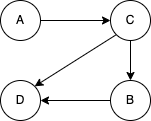
\includegraphics[width=5cm, height=4cm]{figuras/01.png}
\end{center}

O Algoritmo implementado teve o seguinte resultado:

\begin{scriptsize}
\estiloR
\begin{lstlisting}[title={Exemplo 01}, label=lst:javacode]
 == Exemplo 01 == 
0 -> 2 -> 3
Caminhos disjuntos encontrados: 1 
\end{lstlisting}
\end{scriptsize}

\subsection{Experimento 02}

Dado o seguinte grafo, devemos encontrar dois caminhos disjuntos, sendo eles [1 $\rightarrow$ 2 $\rightarrow$ 4] e [1 $\rightarrow$ 3 $\rightarrow$ 4]

\begin{center}
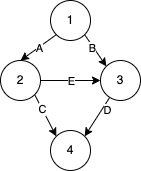
\includegraphics[height=4cm]{figuras/02.png}
\end{center}

O Algoritmo implementado teve o seguinte resultado:

\begin{scriptsize}
\estiloR
\begin{lstlisting}[title={Exemplo 02}, label=lst:javacode]
 == Exemplo 02 == 
0 -> 1 -> 3
0 -> 2 -> 3
Caminhos disjuntos encontrados: 2 
\end{lstlisting}
\end{scriptsize}

\subsection{Experimento 03}

Dado o seguinte grafo, devemos encontrar três caminhos disjuntos, sendo eles [1 -> 2 -> 8] e [1 -> 5 -> 8] e [1 -> 3 -> 7 -> 8]

\begin{center}
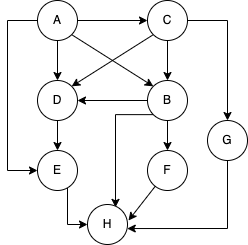
\includegraphics[height=4cm]{figuras/03.png}
\end{center}

e o grafo desenhado com os caminhos que devem ser encontrados:

\begin{center}
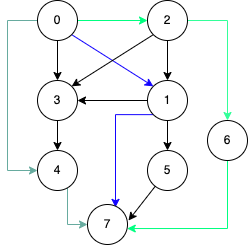
\includegraphics[height=6cm]{figuras/03_caminhos.png}
\end{center}


O Algoritmo implementado teve o seguinte resultado:

\begin{scriptsize}
\estiloR
\begin{lstlisting}[title={Exemplo 03}, label=lst:javacode]
 == Exemplo 03 == 
0 -> 1 -> 7
0 -> 4 -> 7
0 -> 2 -> 6 -> 7
Caminhos disjuntos encontrados: 3 
\end{lstlisting}
\end{scriptsize}


\subsection{Experimento 04}

Dado o seguinte grafo, devemos encontrar dois caminhos disjuntos, sendo eles 
[0 -> 1 ]

\begin{center}
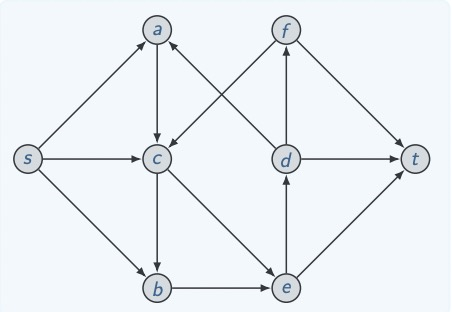
\includegraphics[height=4cm]{figuras/04.jpg}
\end{center}

e o grafo desenhado com os caminhos que devem ser encontrados (conforme no slide da aula):

\begin{center}
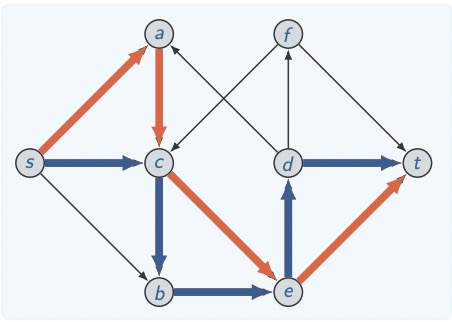
\includegraphics[height=6cm]{figuras/04_caminhos.jpg}
\end{center}

entretanto, o algoritmo encontrou outros possíveis caminhos:

\begin{center}
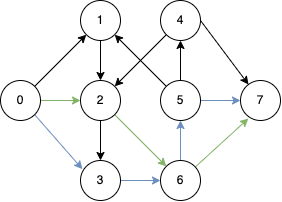
\includegraphics[height=6cm]{figuras/04_caminhos2.png}
\end{center}



O Algoritmo implementado teve o seguinte resultado:

\begin{scriptsize}
\estiloR
\begin{lstlisting}[title={Exemplo 04}, label=lst:javacode]
 == Exemplo 04 == 
0 -> 2 -> 6 -> 7
0 -> 3 -> 6 -> 5 -> 7
Caminhos disjuntos encontrados: 2 
\end{lstlisting}
\end{scriptsize}


\section{Resultados Obtidos}

Implementei um algoritmo usando a base do Fork-Fulkerson com grafo residual e pesos 0 nas arestas para que não haja repetição das mesmas e uma busca em largura como um algoritmo de busca para encontrar os caminhos, seguindo pela lógica arestas ja visitadas e pesoso para um possível futura implementação nesse código.

O algoritmo está funcionando, vários testes foram feitos, inclusive utilizando um problema apresentado em aula chegando também em dois caminhos disjuntos diferentes, mas possíveis dentro do problema em questão.


%%%%%%%%%%%%%%%%%%%%%%%%%%%%%%%%%%%
%% FIM DO TEXTO
%% Inicio da Bibliografia
%%%%%%%%%%%%%%%%%%%%%%%%%%%%%%%%%%%

%%\selectlanguage{brazilian}
% \newpage
% \singlespace{
%     \renewcommand\refname{REFERÊNCIAS}
%     %\bibliographystyle{abnt-alf}
%     \bibliography{bibliografia}
% }

\end{document}